\subsection{Random Forest}
\label{subsubsec:eda_rf}

Random Forest es un algoritmo de aprendizaje automático basado en la combinación de múltiples árboles de decisión, propuesto por Leo Breiman en 2001 ~\parencite{2001randomforest}. Pertenece a la familia de métodos \textit{ensemble}, que mejoran el rendimiento agregando las predicciones de varios modelos más simples.

\subsubsection*{Arquitectura y funcionamiento}

El algoritmo construye un ``bosque'' (conjunto) de árboles de decisión donde cada árbol se entrena de forma ligeramente diferente, introduciendo aleatoriedad controlada en dos niveles:

\begin{itemize}
    \item \textbf{Bootstrap aggregating (bagging)}: Cada árbol se entrena con una muestra aleatoria del conjunto de datos original, permitiendo repeticiones.
    
    \item \textbf{Selección aleatoria de características}: En cada división de un nodo del árbol, solo se considera un subconjunto aleatorio de todas las características disponibles.
\end{itemize}

\subsubsection*{Proceso de clasificación}

Cuando llega una nueva muestra de audio con sus características, cada árbol del bosque realiza su propia clasificación. La predicción final se decide por mayoría:

\begin{itemize}
    \item Si la mayoría de los árboles clasifican el audio como deepfake, la predicción final es deepfake.
    \item Si la mayoría lo clasifica como real, la predicción final es real.
\end{itemize}

Este mecanismo de votación reduce drásticamente la varianza del modelo: aunque un árbol individual pueda cometer errores, el consenso del bosque suele ser acertado. Esto se puede ver en la \autoref{fig:voto_mayoria}

\subsubsection*{Hiperparámetros}

Vamos a hablar de los hiperparámetros centrales de Random Forest:

\begin{itemize}
	\item \textbf{n\_estimators}: Define la cantidad de árboles de decisión que conforman el bosque aleatorio. 
	
	\item \textbf{max\_depth}: Controla la profundidad máxima que pueden alcanzar los árboles individuales dentro del bosque.
	
	\item \textbf{min\_samples\_split}: Determina el número mínimo de muestras requeridas para dividir un nodo interno durante la construcción del árbol.
\end{itemize}

\subsubsection*{Ventajas específicas para detección de deepfakes}

Veamos cuáles son algunas de las ventajas de los Random Forest para detección de $deepfakes$:

\begin{itemize}
    \item \textbf{Robustez ante ruido}: Las características de audio pueden contener variaciones por condiciones de grabación; Random Forest maneja bien estos datos ruidosos.
    
    \item \textbf{No requiere normalización}: A diferencia de Redes Neuronales o SVM, no es necesario escalar las características, lo que simplifica el pipeline.
    
    \item \textbf{Resistencia al sobreajuste}: La combinación de $bagging$ y aleatoriedad evita que el modelo memorice el conjunto de entrenamiento.
\end{itemize}

\begin{figure}
	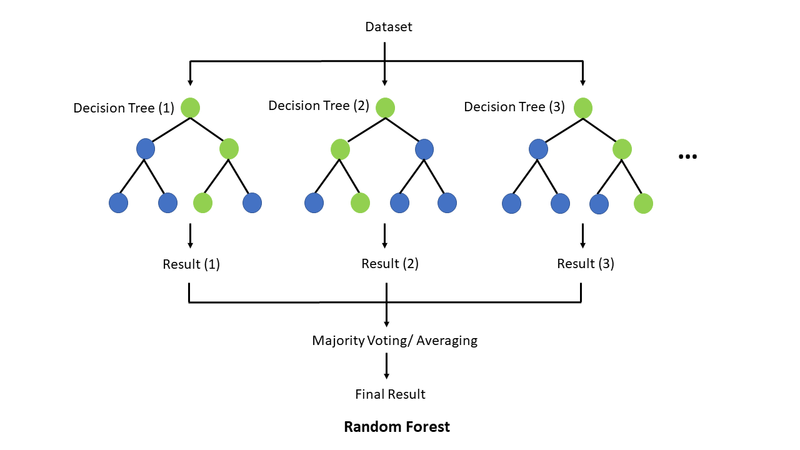
\includegraphics[width=\textwidth]{imagenes/random_forest_majority_vote.png}
	\caption{Voto por mayoría en el ``bosque''.}
	\label{fig:voto_mayoria}
\end{figure}